Dada la siguiente topología:
  \begin{figure}[h]
    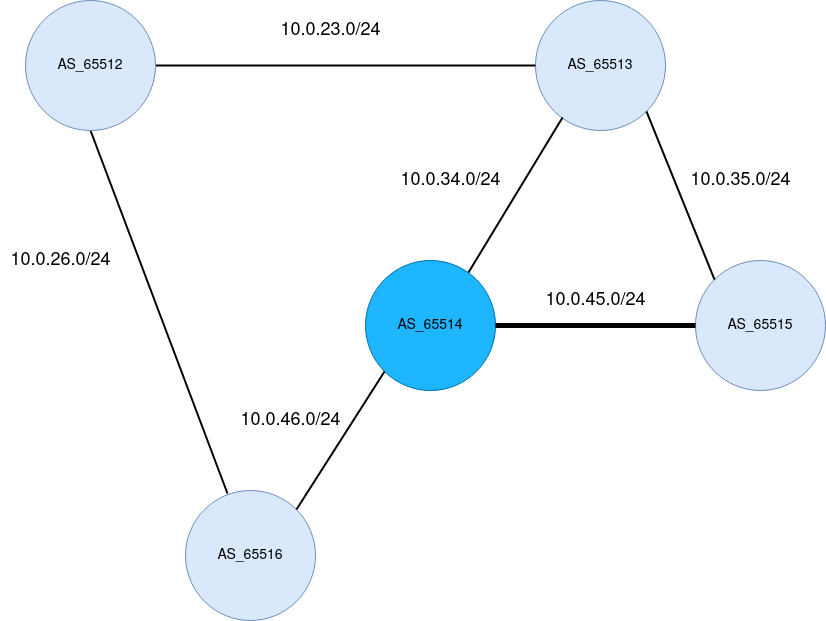
\includegraphics[width=\textwidth]{route-map.png}
  \end{figure}

  \begin{itemize}
    \item El AS65514 desea usar preferentemente su enlace con AS65515,
    y mantener los otros dos como respaldo (backup)
    \item Implementar esa política mediante el uso de \texttt{route-map} .
  \end{itemize}

  Detalles a tener en cuenta:

  \begin{itemize}
    \item Redes de usuario:
    \begin{itemize}
      \item IPv4: 172.16.X.0/24
      \item IPv6: 2001:db8:X::/64
    \end{itemize}
  \end{itemize}

  \[ \forall X \in \{12,13,14,15,16\} \]